%==============================================================================
%  InGARSS 2026 -- Track 06: Machine Learning & AI for Digital Earth
%  Probabilistic, physics-informed forecasting of the combined NOx-O3 hazard.
%
%  Compile: pdflatex main -> bibtex (NOT needed; uses thebibliography) -> pdflatex x2
%  Recommended: Overleaf (IEEEtran is preinstalled) or MiKTeX/TeX Live.
%
%  INTEGRITY: every quantitative value below is transcribed verbatim from
%  RESULTS_LOG.md (the project's single source of truth, CLAUDE.md sec.1).
%  Margin tags "% src:" name the originating run id. No placeholder numbers.
%==============================================================================
\documentclass[conference]{IEEEtran}
\IEEEoverridecommandlockouts

\usepackage{cite}
\usepackage{amsmath,amssymb,amsfonts}
\usepackage{graphicx}
\usepackage{booktabs}
\usepackage{array}
\usepackage{textcomp}
\usepackage{xcolor}
\usepackage[hidelinks]{hyperref}
\usepackage{stfloats}      % allow figure* at bottom of page
\usepackage{dblfloatfix}   % place double-column floats in order (no end-piling)

\graphicspath{{figures/}}

% --- camera-ready space economy (tighten spacing around floats) ---
\setlength{\textfloatsep}{6pt plus 2pt minus 2pt}
\setlength{\floatsep}{6pt plus 2pt minus 2pt}
\setlength{\intextsep}{6pt plus 2pt minus 2pt}
\setlength{\dbltextfloatsep}{6pt plus 2pt minus 2pt}

% chemical-species shorthands
\newcommand{\nox}{\ensuremath{\mathrm{NO_x}}}
\newcommand{\othree}{\ensuremath{\mathrm{O_3}}}
\newcommand{\notwo}{\ensuremath{\mathrm{NO_2}}}
\newcommand{\ox}{\ensuremath{\mathrm{O_x}}}

\begin{document}

\title{Probabilistic Forecasting of the Combined \nox--\othree\ Hazard over
Bangladesh with a Quantile Physics-Informed Neural Network}


\author{
  \begin{tabular}{ccc}
    1\textsuperscript{st} Bishwadip Maitra & 2\textsuperscript{nd} Laboni & 3\textsuperscript{rd} provat sir \\
    \textit{Air-Quality Research Group} & \textit{Air-Quality Research Group} & \textit{Air-Quality Research Group} \\
    \textit{ BUET, Bangladesh} & \textit{BUET, Bangladesh} & \textit{BUET, Bangladesh} \\
    \small bishwadip.maitra@buet.ac.bd & \small author2@buet.ac.bd & \small author3@buet.ac.bd \\[0.15cm]
  \end{tabular}
  \\
  \begin{tabular}{cc}
    4\textsuperscript{th} mokhkes sir & \qquad\qquad 5\textsuperscript{th} Subhojit Mandal \\
    \textit{Air-Quality Research Group} & \qquad\qquad \textit{Wadhwani School of Data Science and AI } \\
    \textit{BUET, Bangladesh} & \qquad\qquad \textit{Indian Institute of Technology Madras,India} \\
    \small author4@buet.ac.bd & \qquad\qquad \small subhojit.m@iiits.in
  \end{tabular}
}


\maketitle

%------------------------------------------------------------------ ABSTRACT
\begin{abstract}
Bangladesh breathes some of the world's most polluted air, and two of its gaseous oxidants---nitrogen
oxides (\nox) and ozone (\othree)---are bound by fast photochemistry, so hours of jointly elevated
exposure recur and are more harmful than either alone. Operational forecasts, however, remain almost
entirely deterministic and single-pollutant. We instead forecast the \emph{full} hourly predictive
distribution, up to 24\,h ahead, of a single combined \nox--\othree\ hazard index, and from it the
probability that the air enters its most-polluted, hazardous upper range. Our quantile-regressive
physics-informed neural network (QR-PINN), trained on three years of hourly observations from nine
stations (2014--2016), is both sharp and trustworthy: it reaches a CRPS of $0.047$ and a Brier score of
$0.110$ for the top-$30\%$ extreme; conformalised quantile regression restores near-nominal $80/90/95\%$
coverage ($0.781/0.892/0.951$) that holds across the full 24\,h horizon; and it transfers to unseen
stations at small cost (leave-one-station-out pinball $+0.025$). With that calibrated forecaster, we put
the embedded photochemistry on trial across four independent tests: the Leighton photostationary state
and total-oxidant (\ox~$=$~\othree~$+$~\notwo) conservation do not sharpen this \othree-led forecast,
which is best at every lead and in the tail. Two attribution methods agree ($r=0.917$) that the skill
lives in recent concentrations and diurnal structure, not the meteorology the chemistry acts on. The
chemistry earns its place instead as interpretability, recovering physically ordered reaction rates and
station-specific emission scales.
\end{abstract}


\begin{IEEEkeywords}
Probabilistic forecasting, physics-informed neural networks, quantile regression,
explainable AI, conformal prediction, air quality, ozone, Bangladesh.
\end{IEEEkeywords}

%================================================================== INTRODUCTION
%================================================================== INTRODUCTION
\section{Introduction}
Bangladesh is among the most polluted countries on Earth, with severe health and economic
costs~\cite{worldbank2022}. Particulate matter dominates the winter inversion
season, but the gaseous oxidants \nox\ and \othree\ pose a distinct, year-round
hazard, and they are not independent. The two are locked in the fast photochemical cycle
$\notwo+h\nu\!\rightarrow\!\mathrm{NO}+\othree$, $\othree+\mathrm{NO}\!\rightarrow\!\notwo$, so that
the total oxidant $\ox=\othree+\notwo$ is approximately conserved through titration and stands in
for their combined burden~\cite{seinfeld2016}. That coupling has a human cost: the extreme
co-occurrence of \othree\ and \notwo\ is more harmful than either pollutant alone~\cite{fu2022}, which
is exactly why the quantity worth forecasting is the \emph{combined} hazard rather than each species
on its own.

Two recent currents make such a forecast conceivable. Operational air-quality prediction has begun to
move from point estimates toward \emph{predictive distributions}, because an exceedance warning is by
nature probabilistic~\cite{perezvasseur2021}. In parallel, physics-informed neural networks
(PINNs)~\cite{raissi2019,karniadakis2021} embed governing equations as soft training constraints, and
have reached air quality through transport-physics graph models~\cite{hettige2024}. These remain
deterministic and single-pollutant, however; the quantile-PINNs~\cite{hu2025} that could close that gap
live only outside the atmospheric domain. To our
knowledge no prior work forecasts a combined \nox--\othree\ hazard probabilistically with embedded
photochemistry, and none does so for Bangladesh.

We set out to fill that gap. Our primary contribution is the forecaster itself: a QR-PINN that emits the
full 24\,h predictive distribution of a balanced, climatology-referenced combined hazard index for
Bangladesh---and, from it, the probability of entering the most-polluted, hazardous upper range---made
trustworthy through calibration-aware learning with conformalised quantile regression and shown to
survive transfer to stations the model never saw. That calibrated forecaster then lets us press a sharper
scientific question---does embedding \nox--\othree\ chemistry actually \emph{improve} a probabilistic
forecast, or only decorate it?---which we answer honestly with independent ablations and a
regime-by-regime audit. Finally, Integrated Gradients and occlusion tell us what the network truly relies
on, and so why the physics pays off where it does and not where it does not.
%================================================================== DATA
\section{Data and Study Area}
Our observations come from nine Department of Environment (DoE) stations across Bangladesh, hourly
from 2014-01-01 to 2016-12-31 (223{,}776 raw rows). The network (Fig.~\ref{fig:overview}a) spans the
Dhaka megacity and its industrial belt (the Bangladesh Agricultural Research Council, BARC, and
Darus~Salam within the city; Gazipur and Narayanganj on its fringes), the port of Chittagong (Agrabad),
and the divisional cities of Khulna, Rajshahi, Sylhet and Barishal, covering markedly different urban
and peri-urban regimes. Both pollutants are sharply right-skewed (Fig.~\ref{fig:overview}b), the
statistical fingerprint of episodic, recurring extremes. Inverse-distance-weighted station-mean
surfaces (Fig.~\ref{fig:overview}c,d) reveal a spatial \textit{anti-structure}: \notwo\ peaks over the
urban core while \othree\ peaks in the cleaner periphery, the same titration chemistry the model must
learn, written across the map.

Each station carries four pollutant channels ($\mathrm{NO}$, \notwo, \nox, \othree) alongside reanalysis
meteorology and physical drivers (temperature, humidity, wind $u/v$, shortwave radiation, boundary-layer
height, ventilation coefficient, photochemical-activity index, surface pressure), daily MODIS fields
(aerosol optical depth, NDVI, fire counts), and calendar terms, 26 features in all. Pollutant gaps are
heavy---\othree\ and \nox\ are populated only about $74.7\%$ and $62.6\%$ of the time---so we keep a
per-channel missingness mask for every input and never impute the target. After quality control and
hourly windowing the modelling tensor is $9\times 26{,}304\times 26$, yielding 86{,}037 training points
(2014--15) and 31{,}067 test points (2016); spatial generalisation is judged by leave-one-station-out
(LOSO).

\begin{figure}[t]
\centering
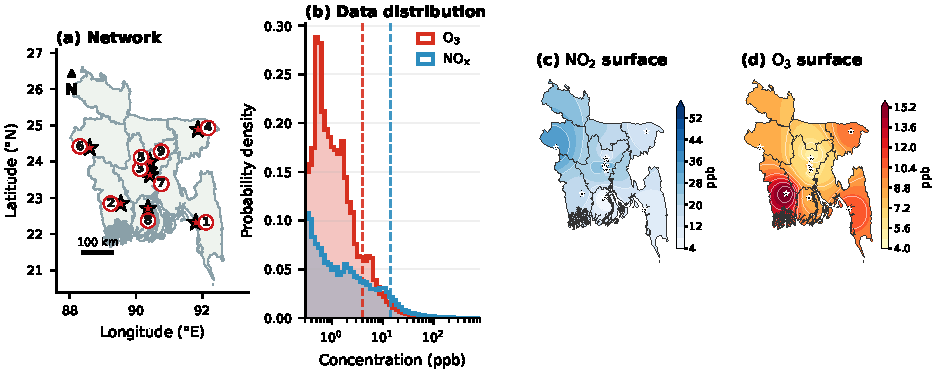
\includegraphics[width=\columnwidth]{fig1_composite.pdf}
\caption{Study area and data. (a)~The nine DoE stations (red stars, numbered 1~Agrabad,
2~Khulna, 3~BARC, 4~Sylhet, 5~Darus~Salam, 6~Rajshahi, 7~Narayanganj, 8~Barishal, 9~Gazipur)
over the eight divisions of Bangladesh. (b)~Pooled distributions (dashed $=$ median): both
pollutants are right-skewed and heavily gapped. (c,d)~Station-mean kriged surfaces (ppb):
\notwo\ peaks over the Dhaka core, \othree\ over cleaner periphery---the spatial fingerprint
of \nox--\othree\ titration motivating a \emph{combined} oxidant target.}
\label{fig:overview}
\end{figure}

\begin{figure*}[t]
\centering
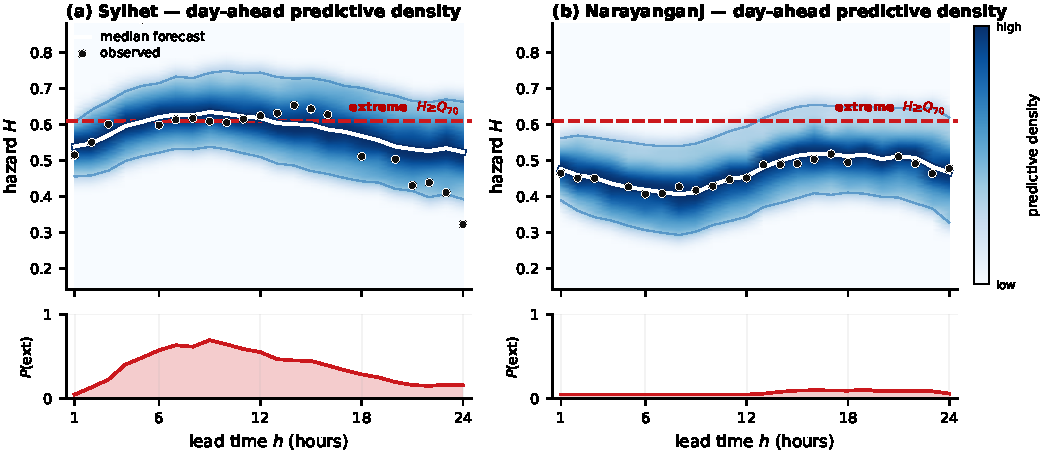
\includegraphics[width=0.85\textwidth]{fig2_forecast.pdf}
\caption{Representative day-ahead forecasts from the data-only QR-PINN (test 2016), shown as the
\emph{full predictive density} of the combined hazard $H$ at each lead (blue ``river''; darker $=$ higher
density), overlaid with the median (white), the observed trajectory (points), the extreme line
$H\!\ge\!Q_{70}$, and the derived exceedance probability $P(\mathrm{ext})\!=\!P(H\!\ge\!Q_{70})$ read off
the predicted CDF (lower strip). (a)~A hazardous build-up at Sylhet: the predictive mass rises across
$Q_{70}$ and the exceedance probability climbs sharply. (b)~A low-risk day at Narayanganj, where the
distribution stays tight and below the extreme line, so $P(\mathrm{ext})\!\approx\!0$. \texttt{src: run E12.}}
\label{fig:forecast}
\end{figure*}

%================================================================== METHOD
\section{Method: A Quantile Physics-Informed Neural Network}

\subsection{Combined hazard index}
A quantile target must be a graded, continuous hazard that is at once physically and health-meaningful,
with neither pollutant allowed to dominate by scale. We therefore adopt a rank, or quantile-uniform,
index
\begin{equation}
H \;=\; \tfrac{1}{2}\,F_{\nox}(\nox) \;+\; \tfrac{1}{2}\,F_{\othree}(\othree),
\label{eq:H}
\end{equation}
where $F_{\bullet}$ is the \emph{training} empirical CDF of each pollutant, so each marginal is uniform
on $[0,1]$. This choice was not cosmetic. An earlier scale-based combination let \othree\ overpower the
index (training variance share \othree~$72.8\%$ vs.\ \nox~$44.1\%$; prediction correlation
\othree~$0.898$ vs.\ \nox~$0.116$), quietly turning a ``combined'' target into an ozone forecast; the
rank form in \eqref{eq:H} rebalances it (variance share $61.0\%/63.3\%$; prediction correlation
\nox~$0.348$, \othree~$0.629$). The combined extreme then follows from a climatology-referenced cutoff,
\begin{equation}
\begin{aligned}
\mathrm{thr}&=Q_{70}(H_{\text{train}})=0.6087,\\
p_{t+h}&=\Pr(H_{t+h}\ge \mathrm{thr}),
\end{aligned}
\label{eq:thr}
\end{equation}
i.e.\ the 70th percentile, so that the \emph{most-polluted top $30\%$} of hours form the
extreme/hazardous class (test base rate $0.263$), with $Q_{90}$ (top $10\%$, base rate $0.046$) marking a
secondary ``severe'' tier. The choice is principled: because the index is rank/quantile-uniform,
$H\!\ge\!Q_{70}$ is by construction the upper tercile of \emph{joint} \nox--\othree\ burden; the joint
upper range of the two oxidants is super-additively harmful~\cite{fu2022} and, in one of the world's most
polluted settings~\cite{worldbank2022}, these are the genuinely hazardous hours, while percentile-based
exceedance is standard practice in probabilistic air-quality forecasting~\cite{perezvasseur2021} and
quantile-regression extremes~\cite{cannon2018}. The model never trains on this binary label; the
exceedance probability $p_{t+h}$ is read directly off the predicted CDF.

\subsection{Architecture and quantile head}
An LSTM encoder (hidden size 64) ingests the 48\,h multivariate window together with a
nine-station embedding (dim.\ 8) and emits a latent state, from which two heads branch
(Table~\ref{tab:arch}).

\begin{table}[t]
\caption{QR-PINN architecture. The monotone quantile head is the deliverable; the physics head is a
regulariser/interpretability device, not an accuracy mechanism.}
\label{tab:arch}
\centering\footnotesize
\renewcommand{\arraystretch}{1.12}
\begin{tabular}{@{}p{0.285\columnwidth}p{0.44\columnwidth}p{0.155\columnwidth}@{}}
\toprule
\textbf{Component} & \textbf{Configuration} & \textbf{Output}\\
\midrule
Input window & 48\,h $\times$ 26 feat.\ $+$ per-channel masks & $\mathbf{x}_t$\\
Station embedding & 9 stations $\rightarrow$ dim.\ 8 & $\mathbf{e}_s$\\
Encoder & LSTM, hidden 64 & latent $\mathbf{z}_t$\\
\textbf{Quantile head} \emph{(deliverable)} & monotone non-crossing, 9\,$\tau$ ($\!\rightarrow\!\{0.01..0.99\}$ tails) & $Q_\tau(H_{t+h})$\\
Physics head & semi-implicit NO--\notwo--\othree\ box-ODE; Leighton $+\,$\ox\ cons.; per-station emission; 9 global rates & $\hat{\mathbf{c}},\,r_{\mathrm{L}}$\\
Loss & pinball $+\,\lambda_{\mathrm{data}}$recon $+\,\lambda_{\mathrm{chem}}r_{\mathrm{L}}$ (annealed) & scalar\\
Output & predictive CDF/PDF; $P(H\!\ge\!\mathrm{thr})$ & $h\!=\!1..24$\\
\bottomrule
\end{tabular}
\end{table}
The \emph{quantile head} (the deliverable) predicts, for each lead $h\!\in\!\{1,\dots,24\}$
and quantile level $\tau$, a value $Q_\tau(H_{t+h})$ trained with the pinball loss
$\rho_\tau(u)=u\,(\tau-\mathbb{1}\{u<0\})$. To forbid quantile crossing we build the
quantiles monotonically from non-negative increments,
\begin{equation}
Q_{\tau_k}=Q_{\tau_1}+\sum_{j=2}^{k}\mathrm{softplus}(\delta_j),\quad \delta_j\in\mathbb{R},
\label{eq:noncross}
\end{equation}
so $Q_{\tau_1}\!\le\!\dots\!\le\!Q_{\tau_K}$ by construction~\cite{cannon2018}.
We train on $\tau\in\{0.05,\dots,0.95\}$ and extend to $\{0.01,\dots,0.99\}$ for tail
calibration. The dense, monotone quantiles define the predictive CDF/PDF per horizon.

\subsection{Embedded physics}
The \emph{physics head} advances per-species concentrations through a coupled box model
at each station. For species $k$ the hourly mass balance is
\begin{equation}
\begin{aligned}
\frac{\mathrm{d}C_k}{\mathrm{d}t}={}&\frac{E_k}{H_{\mathrm{mix}}}
-\frac{V_C}{H_{\mathrm{mix}}}C_k-\frac{v_{d,k}}{H_{\mathrm{mix}}}C_k\\
&-\,\Lambda_k P\,C_k+R_k,
\end{aligned}
\label{eq:box}
\end{equation}
with emission $E_k$, mixing height $H_{\mathrm{mix}}$, ventilation $V_C$, deposition
$v_{d,k}$, wet scavenging $\Lambda_k P$, and chemistry $R_k$. The \nox--\othree\ coupling
enters as two residual penalties, the Leighton photostationary state and \ox\ conservation,
\begin{equation}
\begin{aligned}
r_{\mathrm{L}}&=C_{\othree}C_{\mathrm{NO}}-\tfrac{J}{k(T)}\,C_{\notwo},\\
\ox&=\othree+\notwo\quad(\text{slowly varying}),
\end{aligned}
\label{eq:chem}
\end{equation}
where $J$ scales with the photochemical-activity index and $k(T)$ is Arrhenius in temperature. Every
rate parameter is global and learnable, so its fitted value becomes an interpretable scientific output
rather than a hidden weight. The full objective combines the distributional fit with the physics as a
soft, annealed regulariser:
\begin{equation}
\begin{aligned}
\mathcal{L}={}&\underbrace{\textstyle\sum_{\tau,h}\rho_\tau(H_{t+h},Q_\tau)}_{\text{pinball (primary)}}
+\lambda_{\mathrm{phys}}\,\mathcal{R}_{\mathrm{box}}\\
&+\lambda_{\mathrm{chem}}(r_{\mathrm{L}}+r_{\ox})+\lambda_{\mathrm{data}}\,\mathcal{R}_{c},
\end{aligned}
\label{eq:loss}
\end{equation}
with $\lambda_{\mathrm{phys}}$ annealed $0\!\rightarrow\!\text{target}$ and
$\lambda_{\mathrm{data}}$ a concentration data-fit term where observed.

%================================================================== EXPERIMENTS
\section{Experimental Design}
A probabilistic forecaster must be judged as a distribution, so we score it with strictly proper
rules~\cite{gneiting2007}: the average pinball loss and the CRPS from the quantile grid. Whether its
stated uncertainty can be trusted is a separate question, answered with prediction-interval coverage
(PICP) and width, PIT recalibration~\cite{kuleshov2018}, and conformalised quantile regression
(CQR)~\cite{romano2019} fit on an early-2016 split and tested on late-2016. Hazard skill is the Brier
score on the exceedance probability $p_{t+h}$ of \eqref{eq:thr}, and spatial robustness comes from LOSO
with a moving-block bootstrap (block $=24$\,h, $B=1000$) for 95\% confidence intervals. To see
\emph{why} the model behaves as it does, we attribute its predictions with Integrated
Gradients~\cite{sundararajan2017} against a completeness-checked ``missing'' baseline and with
model-agnostic occlusion~\cite{fisher2019} in the model's own loss, reporting the two together because
saliency on time series is unreliable alone~\cite{ismail2020}. Every number below is transcribed from the
project results log.

%================================================================== RESULTS
\section{Results and Discussion}

\subsection{A target that is genuinely combined}\label{ssec:combined}
Before trusting the forecast we had to trust the target. The first version of $H$ scaled each pollutant
and added them, but ozone's wider spread let it hijack the combination, and the model's prediction then
correlated with \othree\ at $0.898$ while barely moving with \nox\ ($0.116$). The rank index
\eqref{eq:H} strips out that scale advantage by construction: it lifts \nox's prediction correlation
from $0.116$ to $0.348$ and evens the variance shares (\S III-A), so the forecast now answers to both
pollutants instead of tracking ozone alone.

\subsection{A calibrated distributional forecaster}\label{ssec:calib}
That the forecaster has real skill is quickly established. On the original index every learned model cut
the pinball loss by about $45\%$ relative to a climatological quantile baseline ($1.05$ vs.\ $1.93$); on
the adopted rank index the data-driven model reaches a CRPS of $0.047$ and a Brier score of $0.110$ for
the top-$30\%$ extreme, and Fig.~\ref{fig:forecast} shows its full predictive density tracking two
representative day-ahead trajectories---the distribution rising across $Q_{70}$ during a hazardous
build-up at Sylhet, and staying tight and below the extreme line on a calm day at Narayanganj. Because
the rank index lives on $[0,1]$, its scores are comparable only within the rank index. Calibration is
the harder test. Raw quantiles
are over-confident, the nominal-$90\%$ interval covering only $0.839$ of outcomes (Fig.~\ref{fig:results}a);
PIT recalibration narrows the gap but leaves the upper tail short, and only CQR returns coverage to
nominal at every level ($80/90/95\%\rightarrow0.781/0.892/0.951$; Table~\ref{tab:calib}) for a modest cost
in width. As a day-ahead product demands, that coverage also holds as the horizon lengthens, staying near
$0.90$ at $h=1,6,12$ and $24$\,h (CQR PICP$_{90}=0.893/0.887/0.902/0.900$; Fig.~\ref{fig:results}a, inset).
These guarantees do not come at the cost of robustness: the forecaster degrades gracefully across lead
time, seed and exceedance threshold, and---most demandingly---across space (Table~\ref{tab:robust}), the
spatial test we turn to next.

\begin{table}[t]
\caption{Interval calibration (rank index, late-2016 eval). CQR attains near-nominal
empirical coverage (PICP) at all levels.\,\textsuperscript{a}}
\label{tab:calib}
\centering\footnotesize
\renewcommand{\arraystretch}{1.05}
\begin{tabular}{@{}lcccc@{}}
\toprule
Nominal & PICP raw & PICP PIT & \textbf{PICP CQR} & width CQR\\
\midrule
0.80 & 0.725 & 0.760 & \textbf{0.781} & 0.208\\
0.90 & 0.839 & 0.875 & \textbf{0.892} & 0.282\\
0.95 & 0.923 & 0.936 & \textbf{0.951} & 0.365\\
\bottomrule
\end{tabular}
\\[2pt]
\raggedright\textsuperscript{a}\,\texttt{src: run E6}. Split-CQR coverage is approximate
under time-series non-exchangeability; adaptive variants~\cite{gibbs2021} are future work.
\end{table}

\begin{figure*}[t]
\centering
\begin{minipage}[t]{0.36\textwidth}\centering
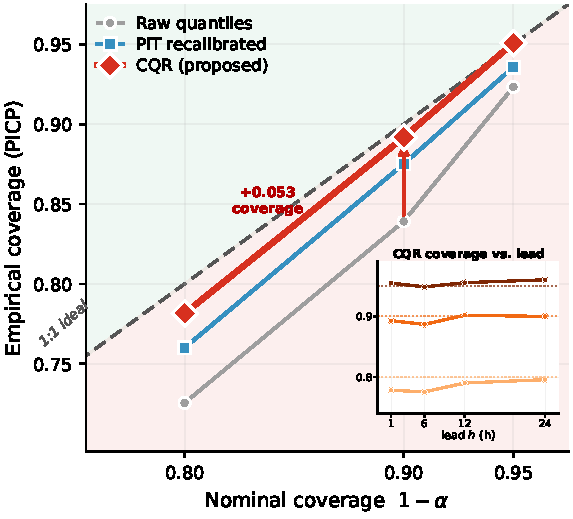
\includegraphics[width=\linewidth]{fig3_reliability.pdf}\\[1pt]
{\footnotesize (a) Interval calibration (reliability)}
\end{minipage}\hspace{0.05\textwidth}%
\begin{minipage}[t]{0.36\textwidth}\centering
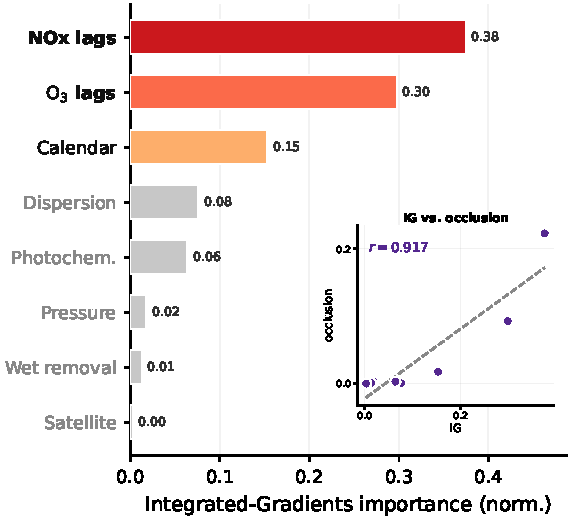
\includegraphics[width=\linewidth]{fig4_importance.pdf}\\[1pt]
{\footnotesize (b) Explainability (group importance)}
\end{minipage}
\caption{Headline results. (a)~Raw quantiles under-cover; PIT helps but leaves the tail short, and CQR
restores near-nominal coverage at all levels and across lead time (inset) (\texttt{src: run E6}).
(b)~Two independent attribution methods agree ($r{=}0.917$) and point to pollutant-lag and calendar
features, not meteorology, as the forecast drivers, which is why the embedded physics adds no accuracy
(\texttt{src: run E9}).}
\label{fig:results}
\end{figure*}

\subsection{Transfer to unseen stations, and robustness}\label{ssec:transfer}
A forecaster is only useful where it has not been trained, so we retrained a station-agnostic QR-PINN and
evaluated it leave-one-station-out. It generalises with a small, well-quantified penalty: LOSO pinball
$0.2277\pm0.0655$ against an in-distribution $0.2024$, a transfer gap of only $+0.0253$. The per-station
errors track how much clean data each fold carries, best on the large Barishal and Narayanganj folds and
worst on the tiny BARC and Gazipur ones, which is exactly the behaviour a single global physics, rather
than regime-clustered parameters, was meant to deliver. The usual spatial cross-validation caveats
apply~\cite{roberts2017}. Spatial transfer is the most demanding of a battery of stress tests
(Table~\ref{tab:robust}): coverage and skill also hold from $h{=}1$ to $24$\,h, are unchanged across
seeds, and persist as the exceedance level rises from $Q_{70}$ to $Q_{90}$---a forecaster that is
\emph{robust}, not merely accurate in-sample.

\begin{table}[t]
\caption{Forecast robustness (data-only QR-PINN, rank index). Skill and calibration hold across lead
time, seed, exceedance threshold, and---most demandingly---spatial transfer.\,\textsuperscript{a}}
\label{tab:robust}
\centering\footnotesize
\renewcommand{\arraystretch}{1.08}
\begin{tabular}{@{}p{0.205\columnwidth}p{0.235\columnwidth}p{0.45\columnwidth}@{}}
\toprule
\textbf{Stress test} & \textbf{Setting} & \textbf{Result}\\
\midrule
Lead time & $h{=}1\!\rightarrow\!24$ & pinball $0.141\!\rightarrow\!0.217$; PICP$_{90}$ $0.893\!\rightarrow\!0.900$\\
Spatial (LOSO) & in-dist\,/\,LOSO & pinball $0.202\,/\,0.228$ (gap $+0.025$)\\
Seed & $s_0\,/\,s_1$ & pinball $0.206\,/\,0.206$ (identical)\\
Threshold & $Q_{70}/Q_{80}/Q_{90}$ & Brier(exc) $0.110\,/\,0.075\,/\,0.034$\\
\bottomrule
\end{tabular}
\\[2pt]
\raggedright\textsuperscript{a}\,\texttt{src:} lead \texttt{E12}, coverage \texttt{E6}, LOSO \texttt{E7},
seed \texttt{E8}, threshold \texttt{THRCORR-Q70}. Rank-index $[0,1]$ metrics (internal comparison); rows
probe distinct robustness axes; exceedance base rates are $0.263/0.134/0.046$ at $Q_{70}/Q_{80}/Q_{90}$.
\end{table}

\subsection{Putting the physics on trial}\label{ssec:phys}
We attacked this question from three independent directions so that no single design choice could be
blamed for the outcome. A physics-weight sweep came first: the
pinball loss barely moved as $\lambda_{\mathrm{phys}}$ rose from $0$ ($0.2054$) to $0.2$ ($0.2063$) and
grew clearly worse at $0.5$ ($0.2188$), with seed-to-seed scatter ($0.2063$ vs.\ $0.2060$) larger than
any physics effect. We then went to the opposite extreme and forced the box-ODE to produce the forecast
on its own, which was far worse ($+0.1375$ pinball). Finally we built the fairest test we could, a
capacity-preserving hybrid in which a neural residual corrects a stable, semi-implicit box-ODE that is
even handed the \emph{observed} future meteorology as forcing; it too trails the free model
(Table~\ref{tab:skill}). The three verdicts agree, and we report them plainly: embedding \nox--\othree\
box chemistry does not improve the probabilistic accuracy of $H$ on this ozone-led target. The failure
is scientific rather than numerical, since the re-engineered ODE is sound: the hybrid ($0.25$) and
physics-only ($0.32$) variants comfortably beat the earlier broken forcing trial ($0.35$), so the model
no longer collapses; it simply does not need the chemistry. A fourth test, a regime-by-regime audit
(\S\ref{ssec:limits}), closes the remaining escape routes: the data-driven forecast wins at every lead,
in the upper tail, and in every input-missingness tier, with no regime in which the physics overtakes it.

\begin{table}[t]
\caption{Forecast skill on the combined index, test 2016 (seed 0).\,\textsuperscript{a}
The data-only model is best; physics is neutral-to-negative.}
\label{tab:skill}
\centering\footnotesize
\renewcommand{\arraystretch}{1.05}
\begin{tabular}{@{}lcccc@{}}
\toprule
Model & Pinball\,$\downarrow$ & CRPS\,$\downarrow$ & Brier(exc)\,$\downarrow$ & PICP$_{90}$\\
\midrule
\textbf{Data-only (free)} & \textbf{0.2099} & \textbf{0.0466} & \textbf{0.1101} & 0.788\\
Hybrid (physics) & 0.2525 & 0.0561 & 0.1376 & 0.826\\
Physics-only & 0.3174 & 0.0705 & 0.1940 & 0.772\\
\bottomrule
\end{tabular}
\\[2pt]
\raggedright\textsuperscript{a}\,Pinball/CRPS/PICP$_{90}$ \texttt{src: run E10}; Brier(exc) at the
corrected $Q_{70}$ extreme cut \texttt{src: THRCORR-Q70}. Rank-index $[0,1]$ metrics (internal comparison
only). Seed-1 reproduces the ordering (free $0.195$, hybrid $0.260$).
\end{table}

\subsection{Why the chemistry is redundant}\label{ssec:xai}
The explanation comes from the attribution analysis, and its credibility rests on agreement rather than
on any single saliency map: Integrated Gradients and occlusion, computed independently, rank the feature
groups almost identically (Pearson $r=0.917$; Fig.~\ref{fig:results}b). Both put the forecast's weight on
recent pollutant lags and the calendar, and find meteorology, photochemistry and satellite inputs nearly
irrelevant. That is precisely why the physics cannot help: the predictable part of $H$ is the ozone and
diurnal signal the network already reads off the lags, whereas the embedded coupling mostly governs the
noisy, traffic-driven \nox\ term. The picture is stable under two further checks, since permuting the
station identity costs almost nothing ($\Delta$pinball $+0.0013$) and the day-night balance of
attribution is nearly flat (\nox-side $0.364$ by day, $0.387$ by night), both consistent with a map
dominated by recent concentrations.

% Figs 3 & 4 are combined side-by-side as Fig.~\ref{fig:results} above.

\subsection{The payoff of the physics, and where it should help}\label{ssec:limits}
If the chemistry does not sharpen accuracy, it earns its keep as interpretation. The fitted parameters
emerge in physically sensible order: learned photolysis ($0.352$) far exceeds titration ($0.057$), the
Arrhenius term is positive, dry deposition orders as $\mathrm{NO}>\notwo>\othree$ ($0.034/0.027/0.021$),
and the per-station emission scales recover real contrasts between the industrial sites and the
residential periphery (one implausible sparse-data scale is excluded). The hybrid forecast even follows
the physics rollout closely (correlation $0.749$). The QR-PINN is therefore best read as a
physics-guided, interpretable forecaster rather than a physics-driven one.

Two boundaries keep this negative result in proportion. The physics variants were handed observed future
meteorology as forcing---an optimistic upper bound---and the rank-index scores are comparable only within
this study. More fundamentally, PINNs help most where data are sparse, noisy or out of
distribution~\cite{raissi2019,karniadakis2021,hettige2024}, and ours is the opposite case: $86{,}037$
hourly points on an ozone-led index whose skill already lives in recent concentrations (\S\ref{ssec:xai}).
Stratifying the free-versus-hybrid gap (\texttt{src: run E12}) confirms the free model wins in every
regime, yet its margin \emph{shrinks} as inputs grow gappier (pinball gap $0.046\!\rightarrow\!0.040$), so
the physics begins to repay where data thin out. Structurally, too, the embedded Leighton cycle is
closed---conserving \ox\ and producing no net \othree---so it can never generate the
VOC/$\mathrm{RO_2}$-driven ozone episodes it is scored against.

%================================================================== CONCLUSION
\section{Conclusion}
We forecast the full day-ahead distribution of a balanced \nox--\othree\ hazard over Bangladesh and
tested whether embedding the underlying photochemistry improves it. The forecaster succeeds: it is well
calibrated, with CQR holding near-nominal coverage across levels and lead times, it transfers to unseen
stations at bounded cost, and it is explainable. The physics, tested four independent ways, does not
improve accuracy on this ozone-led index; the attribution analysis shows why, since the skill resides in
pollutant-lag and calendar structure, not the meteorological drivers the chemistry acts on. We report
that negative result openly and let the physics stand as a source of interpretability.

The same analysis points the way forward. The embedded chemistry should be completed, not abandoned: a
VOC/$\mathrm{RO_2}$ proxy such as the satellite formaldehyde-to-\notwo\ ratio would give the closed
Leighton cycle the net-ozone pathway it now lacks (\S\ref{ssec:limits}), and a graph advection--diffusion
coupling across stations~\cite{hettige2024} could replace the per-station box where data are scarce. The
calibration should move to adaptive conformal inference~\cite{gibbs2021} and shed the perfect-meteorology
forcing assumption.

\section*{Acknowledgments}
The authors thank the Department of Environment (DoE), Bangladesh, for the Continuous Air Monitoring Station (CAMS) data. Claude Opus 4.8 was used for language editing and code optimization.


%================================================================== REFERENCES
\scriptsize
\begin{thebibliography}{00}
\setlength{\itemsep}{0pt}\setlength{\parsep}{0pt}\setlength{\parskip}{0pt}
\bibitem{worldbank2022} World Bank, \emph{Breathing Heavy: New Evidence on Air Pollution
and Health in Bangladesh}. Washington, DC: World Bank, 2022.
\bibitem{seinfeld2016} J. H. Seinfeld and S. N. Pandis, \emph{Atmospheric Chemistry and
Physics}, 3rd ed. Hoboken, NJ: Wiley, 2016.
\bibitem{fu2022} Y. Fu, W. Zhang, Y. Li, H. Li, F. Deng, and Q. Ma, ``Association and
interaction of $\mathrm{O_3}$ and $\mathrm{NO_2}$ with emergency room visits for
respiratory diseases in Beijing, China: a time-series study,'' \emph{BMC Public Health},
vol.~22, art.~2265, 2022, doi:10.1186/s12889-022-14473-2.
\bibitem{perezvasseur2021} S. P\'erez Vasseur and J. L. Aznarte, ``Comparing quantile
regression methods for probabilistic forecasting of $\mathrm{NO_2}$ pollution levels,''
\emph{Sci. Rep.}, vol.~11, art.~11592, 2021, doi:10.1038/s41598-021-90063-3.
\bibitem{raissi2019} M. Raissi, P. Perdikaris, and G. E. Karniadakis, ``Physics-informed
neural networks: a deep learning framework for solving forward and inverse problems
involving nonlinear PDEs,'' \emph{J. Comput. Phys.}, vol.~378, pp.~686--707, 2019,
doi:10.1016/j.jcp.2018.10.045.
\bibitem{karniadakis2021} G. E. Karniadakis \emph{et al.}, ``Physics-informed machine
learning,'' \emph{Nat. Rev. Phys.}, vol.~3, pp.~422--440, 2021,
doi:10.1038/s42254-021-00314-5.
\bibitem{hettige2024} K. H. Hettige \emph{et al.}, ``AirPhyNet: harnessing physics-guided
neural networks for air quality prediction,'' in \emph{Proc. ICLR}, 2024,
arXiv:2402.03784.
\bibitem{hu2025} H. Hu, Q. Cheng, S. Guo \emph{et al.}, ``A framework for parameter
estimation and uncertainty quantification in systems biology using quantile regression and
physics-informed neural networks,'' \emph{Bull. Math. Biol.}, vol.~87, 2025,
doi:10.1007/s11538-025-01439-9.
\bibitem{cannon2018} A. J. Cannon, ``Non-crossing nonlinear regression quantiles by
monotone composite quantile regression neural network, with application to rainfall
extremes,'' \emph{Stoch. Environ. Res. Risk Assess.}, vol.~32, pp.~3207--3225, 2018,
doi:10.1007/s00477-018-1573-6.
\bibitem{gneiting2007} T. Gneiting and A. E. Raftery, ``Strictly proper scoring rules,
prediction, and estimation,'' \emph{J. Amer. Statist. Assoc.}, vol.~102, no.~477,
pp.~359--378, 2007, doi:10.1198/016214506000001437.
\bibitem{kuleshov2018} V. Kuleshov, N. Fenner, and S. Ermon, ``Accurate uncertainties for
deep learning using calibrated regression,'' in \emph{Proc. ICML}, 2018, arXiv:1807.00263.
\bibitem{romano2019} Y. Romano, E. Patterson, and E. J. Cand\`es, ``Conformalized quantile
regression,'' in \emph{Adv. Neural Inf. Process. Syst. (NeurIPS)}, 2019, arXiv:1905.03222.
\bibitem{gibbs2021} I. Gibbs and E. J. Cand\`es, ``Adaptive conformal inference under
distribution shift,'' in \emph{NeurIPS}, 2021, arXiv:2106.00170.
\bibitem{sundararajan2017} M. Sundararajan, A. Taly, and Q. Yan, ``Axiomatic attribution
for deep networks,'' in \emph{Proc. ICML}, PMLR 70, pp.~3319--3328, 2017, arXiv:1703.01365.
\bibitem{fisher2019} A. Fisher, C. Rudin, and F. Dominici, ``All models are wrong, but many
are useful: learning a variable's importance by studying an entire class of prediction
models simultaneously,'' \emph{J. Mach. Learn. Res.}, vol.~20, no.~177, pp.~1--81, 2019.
\bibitem{ismail2020} A. A. Ismail, M. Gunady, H. Corrada Bravo, and S. Feizi,
``Benchmarking deep learning interpretability in time series predictions,'' in
\emph{NeurIPS}, 2020, arXiv:2010.13924.
\bibitem{roberts2017} D. R. Roberts \emph{et al.}, ``Cross-validation strategies for data
with temporal, spatial, hierarchical, or phylogenetic structure,'' \emph{Ecography},
vol.~40, no.~8, pp.~913--929, 2017, doi:10.1111/ecog.02881.
\end{thebibliography}

\end{document}
